\begin{document}
	The NMOS common source amplifer for this lab was constructed using 2N7000 NMOS transistors. The circuit essentially consists of two parts, the voltage amplifier stage and the current mirror. The generic circuit for the current driver is shown in Figure \ref{fig:currentgeneric}. 
	
	\begin{figure}[H]
		\centering
		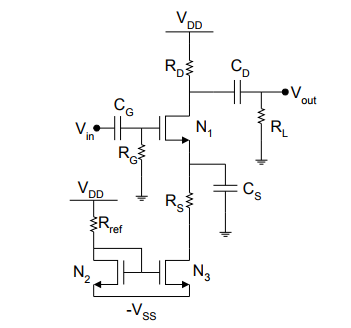
\includegraphics[width=.55\textwidth]{CircuitDevelopment/genericschem.png}
		\caption{Generic common source amplifier circuit \cite{b1}}
		\label{fig:currentgeneric}
	\end{figure}
	
	In order to understand the operation of the circuit, DC analysis of the circuit is required. At DC all the capacitors behave as shorts. It is known that the current through a MOSFET is seen in Equation \ref{eq:k}
	\begin{equation}\label{eq:k}
	I_D = k(V_{gs}-V_t)^2,
	\end{equation}
	
	Where k is the transconductance parameter, V$_{gs}$ is the gate-source voltage and V$_T$ is the threshold voltage. From the datasheet \cite{NMOS},  I$_D$ is 75 mA when V$_{gs}$ is 4.5 V. From Equation \ref{eq:k} k can be found to be 8.5 mA/V. Again using Equation \ref{eq:k}, the corresponding V$_{gs}$ for a bias current of 1 mA is found to be 1.85 V. 
	Upon finding the voltage drop over the NMOS, the source resistance can then be found by KCL across the amplifier NMOS. R$_{s}$ is found to be 8.3 k$\Omega$, R$_{ref}$ can found to be 22.2 k$\Omega$. The capacitor values are chosen such that their impendence is less than their corresponding resistor values. The impendence of the capacitor can be found by Equation \ref{eq:capz}
	
	\begin{equation}\label{eq:capz}
	Z_c = \frac{1}{j\omega C},
	\end{equation}
	
	where $\omega$ is the angular frequency of the input signal in rad/s. By setting Z$_c$ to be less than the corresponding R values, C can be solved to be 4.7 $\mu$F.
	
	
	 AC analysis of the circuit is then required in order to find the drain resistance. Figure \ref{fig:smallsignalnmos} shows the equivalent small signal model for the NMOS.
	
	
	\begin{figure}[H]
		\centering
		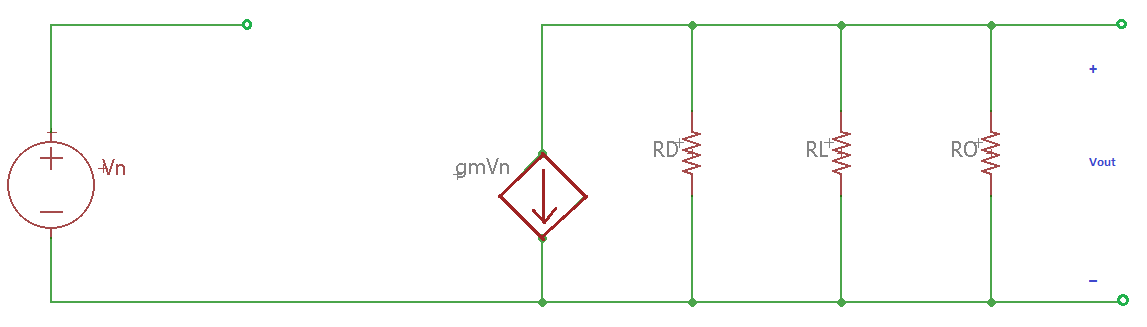
\includegraphics[width=.55\textwidth]{CircuitDevelopment/smallsignal.png}
		\caption{Equivalent small signal circuit}
		\label{fig:smallsignalnmos}
	\end{figure}
	
	The transconductance of this circuit is defined as Equation \ref{eq:trancond}
	
	\begin{equation}\label{eq:trancond}
	g_m = \frac{2I_D}{V_{ov}},
	\end{equation}
	
	where V$_{ov}$ is the overdrive voltage. From this small signal transconductance is found to be 2.8 mA. The small signal r$_0$, defined as Equation \ref{eq:smallro}
	
	\begin{equation}\label{eq:smallro}
	
	r_o = \frac{1}{\lambda I_{DS}},
	
	\end{equation}
	
	where $\lambda$ is the body effect, and found from the datasheet \cite{NMOS} to be zero for the operating conditions. The open circuit gain can then be found by Equation \ref{eq:opengain} 
	
	\begin{equation}\label{eq:opengain}
	\frac{v_o}{v_{in}} = g_mR_o,
	\end{equation}
	
	where R$_o$ is the equivalent resistance of (R$_D$ || R$_L$). The load resistance is provided by the lab, but for this calculation can be assumed to nearly infinite, therefore R$_D$ is found to be around 2 k$\Omega$. The circuit was then simulated in NGSpice integrated with Matlab. The simulated circuit can be seen in Figure \ref{fig:NMOSsimcircuit}.
	
	\begin{figure}[H]
		\centering
		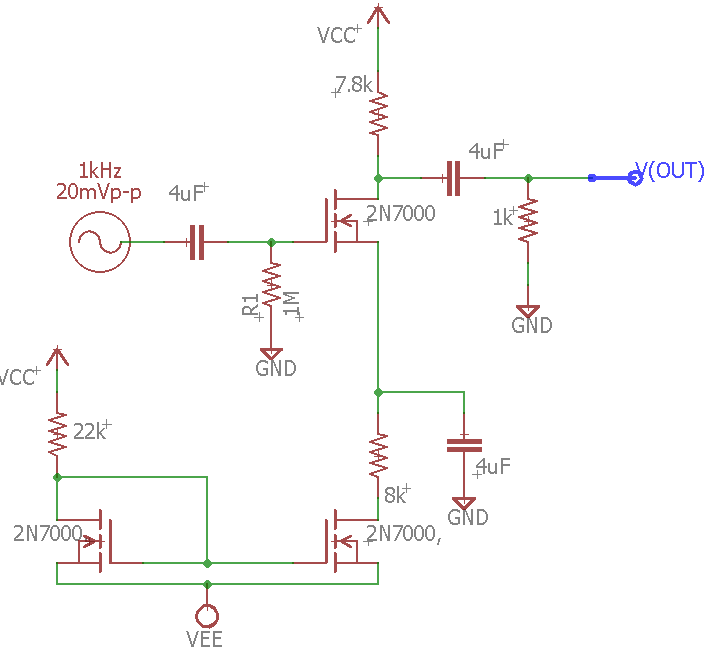
\includegraphics[width=.55\textwidth]{CircuitDevelopment/NMOS_sim.png}
		\caption{Simulated common source amplifier circuit}
		\label{fig:NMOSsimcircuit}
	\end{figure}

	A significant change was required in order to meet specs, the R$_D$ value calculated was off by a factor of 4. This is due to assumptions made during analysis, more detail is provided in discussion. In addition, the negative bias voltage was altered to -8 V in order to reduce harmonic distortion. The frequency of the NMOS is shown in Figure \ref{fig:NMOSfreq}.
	
\begin{figure}[H]
		\centering
		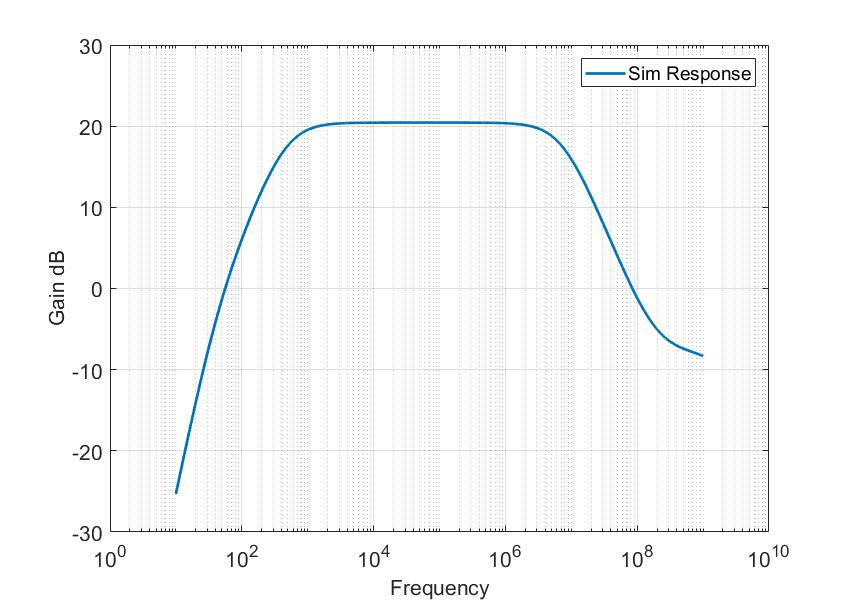
\includegraphics[width=.55\textwidth]{CircuitDevelopment/NMOS_bandwidth.jpg}
		\caption{Simulated frequency response of NMOS amplifier}
		\label{fig:NMOSfreq}
\end{figure}

	The NMOS met the specified gain at 21 dB with a 3dB lower cut off frequency well below the required 1 kHz. The FFT of NMOS can be seen in Figure \ref{fig:nmosfft}.

\begin{figure}[H]
	\centering
	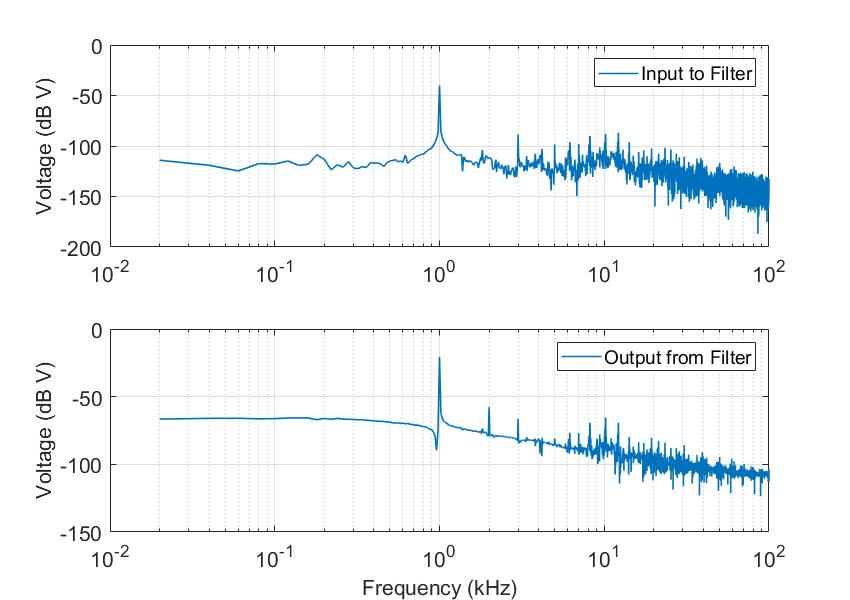
\includegraphics[width=.55\textwidth]{CircuitDevelopment/nmos_FFT.jpg}
	\caption{Simulated FFT of second harmonic distortion}
	\label{fig:nmosfft}
\end{figure}

	This analysis was performed by inputting a 10 mV signal at 1 kHz. The measured distortion on the second harmonic is required to be less than 2\%. By inspection the distortion is found to be 1.5\%. Table \ref{tab:nmossum} summarizes the NMOS simulation results.
	
	
	\begin{table}[H]
		\centering
		\caption{NMOS summary}
		\begin{tabular}{cc}
			$Q_1, Q_2, Q_3$ & 2N7000        \\ \hline
			$R_ref$         & 19.3 k$\Omega$ \\ \hline
			$R_D$           & 7.8 k$\Omega$  \\ \hline
			$R_S$           & 8 k$\Omega$   \\ \hline
			$R_G$           & 1 M$\Omega$  \\ \hline
			$C_g$, $C_d$, $C_l$ & 4.7 $\mu$F   \\ \hline
			Lower cutoff    &  500 Hz \\    \hline
			Upper cutoff    & 10 MHz \\    \hline
			
			     
		\end{tabular}
	\end{table}

After making slight alterations the circuit worked correctly in simulations.
	
	
	
\end{document}	
	